% !TEX root = Formulaire_fluides.tex

\appendix

\section{Propriétés physiques des fluides les plus courants}

\subsection{Valeurs de référence  pour l'eau et l'air}
\vspace{.5cm}
(pour  $T = 20^o C$ ; $P = 10^5 Pa = 1 atm$)

\begin{tabular}{|l|l|l|l|} 
\hline
					& Air 							& Eau pure 						& Eau de mer \\
\hline
Masse volumique & 		$\rho = 1.205 kg/m^3$				& $997,05 kg/m^3$					&  $\rho = 1027 kg/m^3$ \\
 Viscosité cin. & 		$\nu = 1.5e-6 m^2/s$ 				& { $\nu = 1.002 \cdot 10^{-6} m /s^2 $ }		&  $\nu = 1.139 10^{-6} m /s^2$ \\
 Viscosité dyn. & 		$\mu = 1.81 \cdot 10^{-5} Pa \cdot s$ 	&  {  $\mu = 0.999 \cdot  10^{-3} Pa \cdot s$ } 	& \\
 compressibilité & 		$\chi_s = 1.4 atm^{-1}$ 				&$\chi_s =  4.9 \cdot 10^{-5} Atm^{-1}$  	& \\
 dilatabilité & 			$ \alpha = 3.4 \cdot 10{-3} K^{-1}$  		& $ \alpha = 1.5 \cdot 10{-4} K^{-1}$  	& \\
 vitesse du son &		$ c = 334 m/s$ 						& $c = 1500 m/s$ 					& \\  
 \hline
\end{tabular}
%La masse volumique de l'eau vaut $\rho_M = 1000 kg/m^3$ pour le modèle
%et $\rho = 1026 kg/m^3$ pour le navire. La viscosité cinématique de l'eau est 
%$\nu_M = 1.139 10^{-6} m /s^2$ pour le modèle et $\nu = 1.188 10^{-6} m /s^2$
%pour le navire.



\subsection{Equation d'état et loi d'état énergétique de l'air}

$ P = \rho r T ; \qquad  c = \sqrt{\gamma r T}.$

$e = c_v T ; \qquad h = c_p T  ; \qquad c_v = \frac{r}{\gamma-1} ; \qquad  c_p = \frac{\gamma r}{\gamma-1}$

$ r = 287 J/K/kg ; \qquad \gamma = 1.405$.


\subsection{Equation d'état de l'eau de mer (IES80)}

La relation d'état IES80 permet  de calculer $\rho$ ($kg /m^3$) en fonction
de $T$ (température en  en $^o C$), $S$ (salinité en $g/kg$), et $P$ (pression en $Bars$). 

Elle est précise (en toute rigueur) pour $-2^oC<T < 40^o C$, $0<S<40g/kg$, 
$0<P<1500 Bars$.

\vspace{.5cm}

{
\tiny

$$
\rho(T,S,P) = \rho_0(T,S) \left/ \left( 1 - \frac{P}{K(T,S,P)} \right) \right.,
$$

avec :

\begin{eqnarray*}
\rho_0(T,S) &=& 999.842594+6.793952\cdot 10^{-2} \times T-9.09529\cdot 10^{-3} \times T^2+1.001685\cdot 10^{-4} \times T^3 -1.120083\cdot 10^{-6} \times T^4 \\
            &+& 6.536332\cdot 10^{-9} \times T^5+8.24493\cdot 10^{-1} \times S-4.0899\cdot 10^{-3} \times T S+7.6438\cdot 10^{-5} \times T^2 S \\
	    &-&8.2467\cdot 10^{-7} \times T^3 S + 5.3875\cdot 10^{-9} \times T^4 S-5.72466\cdot 10^{-3} \times S^{1.5}+1.0227\cdot 10^{-4} \times T S^{1.5}\\
	    &-&1.6546\cdot 10^{-6} \times T^2 S^{1.5}+4.8314\cdot 10^{-4} \times S^2, 
\end{eqnarray*}

et 

\begin{eqnarray*}
K(T,S,P) &=& 19652.21+148.4206 \times T-2.327105 \times T^2+1.360447\cdot 10^{-2} \times T^3-5.155288\cdot 10^{-5} \times T^4 \\
         &+&3.239908 \times P+1.43713\cdot 10^{-3} \times T P+1.16092\cdot 10^{-4} \times T^2 P-5.77905\cdot 10^{-7} \times T^3 P \\
         &+&8.50935\cdot 10^{-5} \times P^2-6.12293\cdot 10^{-6} \times T P^2+5.2787\cdot 10^{-8} \times T^2 P^2 \\
         &+&54.6746 \times S-0.603459 \times T S+1.09987\cdot 10^{-2} \times T^2 S \\
         &-&6.1670\cdot 10^{-5} \times T^3 S+7.944\cdot 10^{-2} \times S^{1.5}+1.6483\cdot 10^{-2} \times T S^{1.5}-5.3009\cdot 10^{-4} \times T^2 S^{1.5} \\
         &+&2.2838\cdot 10^{-3} \times P S-1.0981\cdot 10^{-5} \times T P S-1.6078\cdot 10^{-6} \times T^2 P S \\
	 &+&1.91075\cdot 10^{-4} \times P  S^{1.5}-9.9348\cdot 10^{-7} \times P^2 S+2.0816\cdot 10^{-8} \times T P^2 S \\
	 &+&9.1697\cdot 10^{-10} \times T^2 P^2 S.
\end{eqnarray*}

}



\subsection{Viscosité de l'eau et de l'air en fonction de la température}

\paragraph{Cas de l'air} :

Loi (expérimentale) de Sutherland : 
$$
\mu = \mu_0 \left( \frac{T}{T_0} \right)^{3/2} \frac{ T_0 + S }{T+S} 
$$
avec les paramètres :
$$
\mu_0 = 	1.716 \times 10^{-5} P.s,  \quad T_0 = 273.15 K , \quad S = 110.4 K
$$

\paragraph{Cas de l'eau pure} :

Loi (expérimentale)  de Vogel :

$$
\mu(T)  = \mu_0 e^{\frac{B}{T-C}}
$$
avec les paramètres : 
$$ 
\mu_0 = 0.0243 Pa\cdot s, \quad B = 578.919 K, \quad C = 137.54 K
$$
 



\begin{landscape}

\section{Tableau des principaux nombres sans dimensions}

On note ici $U$, $L$ les échelles de vitesse et de longueur du problème, et (pour les problèmes instationnaires) $T$ l'échelle de temps (période) et $f = 1/T$ la fréquence associée.
% (par exemple l'inverse de la fréquence d'oscillation).

\vspace{.5cm}

\begin{tabular}{|l   |l    |c  |c    |l   |}
\hline
Nom & Définition & Signification &Autre interprétation &  Utilité \\
\hline 
\hline
&&&&\\
Knudsen & 
$Kn = \frac{\ell}{L}$ & 
$\displaystyle\frac{ \mbox{échelle microscopique}}{ \mbox{échelle macroscopique}}$ & &
Validité de la MMC
\\
&&&&\\
\hline
&&&&\\
Reynolds & $Re = \frac{U L}{\nu} $& 
$\displaystyle\frac{ \mbox{Convection}}{ \mbox{Frottement visqueux}}$ &
$\displaystyle\frac{ \mbox{Temps caractéristique de convection}}{ \mbox{Temps caractéristique de diffusion}}$
 &
Général
\\
&&&&\\
\hline
&&&&\\
Mach & $Ma = \frac{U }{c}$ & 
$\displaystyle\frac{ \mbox{Convection }}{ \mbox{Compressibilité}}$  &
$\displaystyle\frac{ \mbox{Vitesse de l'écoulement}}{ \mbox{vitesse du son}}$  &
Aérodynamique
\\
&&&&\\
\hline
&&&&\\
Froude & $Fr = \frac{U }{\sqrt{gL}}$ & 
 $\left( \displaystyle \frac{ \mbox{accélération de l'écoulement}}{ \mbox{accélération de gravité}} \right)^{1/2}$  &
  $\displaystyle \frac{ \mbox{Vitesse de l'écoulement}}{ \mbox{Vitesse des ondes de gravité}}$
  &
Hydrodynamique, écoulements à surface libre
\\
&&&&\\
\hline
&&&&\\
Bond
  & $Bo = \frac{L}{\sqrt{\gamma/\rho g}}$  & 
$\displaystyle {\frac{ \mbox{Pesanteur}}{ \mbox{Capillarité}}}$ & 
$ \displaystyle{\frac{ \mbox{Echelle de longueur du problème}}{ \mbox{Longueur capillaire}}}$ 
&
Phénomènes capillaires
\\
(ou E\"otv\"os) &&&&\\
%\hline
%&&&&\\
%Gallilée & $Ga = \frac{\sqrt{g L^3}}{\nu}$ & 
%$\displaystyle\frac{ \mbox{Effets de gravité}}{ \mbox{Effets visqueux}}$ &
%Objets en mouvement libre dans un fluide
%\\
%&&&\\
\hline
&&&&\\
Stokes
 & $St =  \frac{L^2}{\nu T } = \frac{f L^2}{\nu }$ & 
%$\displaystyle \frac{\mbox{Temps  de diffusion visqueuse}}{ \mbox{Période}}$ 
$\displaystyle \frac{ \mbox{Instationarité}}{\mbox{Frottement visqueux}}$ 
&
${\left( \displaystyle\frac{ \mbox{Echelle de longueur du problème}}{ \mbox{Longueur de diffusion visqueuse}}  \right)}^2$ 
&
Ecoulements visqueux instationnaires
\\
(ou Womerseley)  &&&&\\
\hline
&&&&\\
Strouhal
 & $Sr  = \frac{f L}{U} =  \frac{L}{U T}$  & 
$\displaystyle\frac{ \mbox{Instationarité}}{ \mbox{Convection}}$ &
$\displaystyle\frac
{ \mbox{Temps caractéristique de convection}}{ \mbox{ Période de lâcher tourbillonnaire }} 
$ 
&
Ecoulements inertiels instationnaires
\\
&&&&\\
\hline
&&&&\\
Helmholtz
 & $H =  \frac{L}{c T} = \frac{f L}{c} $ & 
$\displaystyle\frac{ \mbox{Echelle de longueur du problème}}{ \mbox{longueur d'onde acoustique}}$ &
$\displaystyle\frac{ \mbox{fréquence caractéristique}}{ \mbox{fréquence acoustique}}$ &

Acoustique
\\
&&&&\\
\hline
\end{tabular}

\end{landscape}



\section{Equations-bilans sous formes locales et intégrales}

Dans cette annexe on résume les équations-bilan de la mécanique des fluides sous forme {\em locale } (equations différentielles gouvernant l'évolution temporelle des quantités locales) puis sous forme {\em intégrale } en considérant un volume de contrôle {\em Fixe} noté $\Omega$ de frontière 
$\partial \Omega$.
On considère ici le cas général d'un fluide soumis à une force {\em massique} $\vec g$ (en général la pesanteur). On ne fait pas d'hypothèse sur le caractère compressible ou incompressible. 
La loi de comportement est dans le cas général (compressible) la loi de Stokes $\mytensor{\tau} = 2 \mu \mytensor{D}'$ avec $ \mytensor{D'} =  ( \mytensor{D} - \divergence ( \vec{u} )\mytensor{I}/3 )$, qui se réduit à la loi de Newton $\mytensor{\tau} = 2 \mu \mytensor{D}$ dans le cas incompressible. On suppose la viscosité $\mu$ constante, 
ainsi que la conductivité thermique $k$.

Il existe de nombreuses variantes de ces équations-bilan, on liste ici les plus utiles. Un grand nombre d'autres formes sont données dans le livre {\em Mécanique des Fluides, Candel (Dunod)}.

%%%%%%%%%%%%%%%%%%%%%%%%%%%%%%
\subsection{Bilan de masse}
\begin{equation}
\mbox{\bf Forme locale 1 (non conservative)  :} 
\qquad  
\ddt{\rho} + \rho \divergence \vec{u} = 0
\end{equation}

\begin{equation}
\mbox{\bf Forme locale 2 (conservative) :}
\qquad  
\dpa{\rho}{t} + \divergence ( \rho \vec{u})  = 0
\end{equation}

\begin{equation}
\mbox{\bf Forme intégrale : } 
\qquad  
\ddt{} \int_{\Omega}  \rho dV = - \oint_{\partial \Omega} \rho \vec{u} \cdot \vec{n} dS
\end{equation}

% % bilan integral, volume matériel
% $$
%\dpdt{} \int_{\Omega} \rho \; dV 
%		=
%		- \oint_{\partial \Omega} \rho \,  \vec{u}\cdot \vec{n} \, dS
%$$

%%%%%%%%%%%%%%%%%%%%%%%%%%%%%%%%%%%%%
\subsection{Bilan de quantité de mouvement}
%\paragraph{Forme locale 1}
\begin{equation}
\mbox{\bf Forme locale 1 (non conservative)  :} 
\qquad  
		\rho \ddt{\vec{u}} 
		= 
		\rho \vec{g}  - \gradient p + \mu \Delta \vec{u} + \frac{\mu}{3} \gradient \divergence \vec{u} 
		%\label{eq:bilan_local_lagrangien_qdm}
\end{equation}
	
	
%\paragraph{Forme locale 2 (conservative)}
%\mbox{\bf Forme locale 2 (conservative) :}
%\qquad  

\begin{equation}
\mbox{\bf Forme locale 2 (conservative) :}
\qquad  
	 \dpa{(\rho \vec{u})}{t} + \divergence (\rho \vec{u} \otimes \vec{u})
		= \rho \vec{g}  - \gradient p + \divergence \mytensor{\tau}
		%\label{eq:bilan_local_lagrangien_qdm}
\end{equation}

\paragraph{Forme intégrale}
	\begin{equation}
		\ddt{} \int_{\Omega} \rho \, \vec{u} \; dV 
		=
		- \oint_{\partial \Omega} \rho \, \vec{u}\; (\vec{u}\cdot \vec{n}) \, dS
		+ \oint_{\partial \Omega} \left( -p \vec{n} + \mytensor{\tau} \cdot \vec{n}\right) \; dS
		+ \int_{\Omega} \rho \vec{g} \, dV 
		\quad { \left[ + \oint_{\cal L} \gamma \vec{n}_{\cal L}  \, d\ell \right]}
		\label{eq:bilan_global_eulerien_qdm}
	\end{equation}
	
{\small (Le dernier terme entre crochets est à prendre en compte si le volume de contrôle $\Omega$ est traversé par une {\em surface libre} ${\cal S}$ ; dans ce cas  $ {\cal L} = {\partial \Omega} \cap \cal S$ et $\vec{n}_{\cal L} $ est le vecteur unitaire contenu dans le plan ${\cal S}$ et perpendiculaire à ${\cal L}$)}

%%%%%%%%%%%%%%%%%%%%%%%%%%%%%
\subsection{Bilan d'énergie cinétique}
%La forme locale s'obtient en projetant le bilan de QDM sur $\vec u$.

\begin{equation}
\mbox{\bf Forme locale 1} \qquad  
		\rho \ddt{} \frac{ |\vec{u}|^2}{2} 
		= 
		\rho \vec{g} \cdot \vec{u}  - \gradient p \cdot {\vec u} + \vec{u} \cdot \divergence ( \mytensor{\tau} )
		%\label{eq:bilan_local_lagrangien_qdm}
\end{equation}

\paragraph{Forme locale 2}

$\,$
Sous les hypothèses suivantes :
\begin{itemize}
\item 
Le champ de force massique $\vec g$ est conservatif, c.a.d. 
$\vec g = -\gradient {\cal U}$ (en général ${\cal U}= g z$), \item  L'écoulement est barotrope ($\rho=\rho(p)$,  ce qui permet de définir la  fonction  ${\cal P} = \int \frac{d p}{\rho}$)\footnote{Cette notion englobe fluide incompressible (avec ${\cal P} = p/ \rho_0$)  ainsi que le gaz parfait en évolution isotherme (avec ${\cal P} = r T_0  \log p $) ou isentropique
 (avec ${\cal P} = \frac{\gamma}{\gamma-1} \frac{p_0}{\rho_0} 
 \left[ \left(\frac{p}{p_0}\right)^{\frac{\gamma-1}{\gamma}} \right] $)
};

\end{itemize}

\begin{equation}
		\rho \dpdt{} \frac{ |\vec{u}|^2}{2} 
		+ \rho \vec{u} \cdot \gradient \left( \frac{ |\vec{u}|^2}{2} + {\cal U} +  {\cal P} \right) 
		= 
		 \vec{u} \cdot \vec{\divergence} ( \mytensor{\tau} ) \quad 
		 %\left( = \divergence ( \vec{u} \cdot \mytensor{\tau} ) - \mytensor{D} :\mytensor{\tau} \right)
		%\label{eq:bilan_local_lagrangien_qdm}
\end{equation}

(on reconnait comme cas particulier le premier théorème de Bernoulli).



\paragraph{Forme intégrale (cas $\vec g$ conservatif) }
	\begin{equation*}
		\underbrace{
		\ddt{} \int_{\Omega}  \left( \frac{\rho |\vec{u}|^2}{2} + \rho {\cal U} \right) \, dV
		}_{\ddt {E_m} }	
		= 
		\underbrace{
		-  \oint_{\partial \Omega} \left( \frac{\rho |\vec{u}|^2}{2} + \rho {\cal U} \right)  \vec u \cdot \vec n \, dS
		}_{\displaystyle \dot E_m^{(ech)} }
		+ 
		\underbrace{
		 \oint_{\partial \Omega}   \vec u \cdot (-p \vec n) \, dS
		}_{\displaystyle \dot W^{(p,ext)} }
		+ 
		\underbrace{
		\int_{\Omega} p \, \divergence (\vec{u}) \, dV 
		}_{\displaystyle \dot W^{(p,int)} }
%+  
%\underbrace{
%\oint_{\partial \Omega}  \vec{u} \cdot \mytensor{\tau} \cdot \vec{n} \, dS
%}_{\displaystyle \dot W^{(v)} }
%\underbrace{
 %-  \int_{\Omega} \myvec{u} \cdot  \mytensor{\tau}  \, dV
 + 
		\underbrace{
		\int_{\Omega}
 \vec{u} \cdot \vec{\divergence} ( \mytensor{\tau} ) \, dV}_{\qquad \quad \displaystyle \dot W^{(v)}  \qquad (9) } 
		\label{eq:bilan_global_eulerien_ec}
	\end{equation*}


où $\displaystyle \dot W^{(v)}$ est la puissance des forces visqueuses,  et 
$\dot E_m^{(ech)}$ le flux convectif d'énergie mécanique.
%\footnote{On ne fait pas à ce stade de distinction entre entre puissance intérieure et puissance extérieure.}


\subsection{Bilan d'énergie (1er principe)}

Dans ce paragraphe $e$ est l'énergie interne {\em volumique}, $h = e+p/\rho$ est l'enthalpie volumique\footnote{ $e = c_v T$ et $h = c_p T$ pour un gaz parfait},  ${\cal E}_{{\cal D}(t)}$ est l'énergie du {\em volume matériel} ${\cal D}(t)$ coïncidant avec $\Omega$ à l'instant $t$, $\cal H$ est l'enthalpie totale du domaine {\em fixe} $\Omega$ , $\vec q$ est le flux de chaleur conductif\footnote{ Donné en général par la loi de Fourier $\vec{q}=-k \gradient T$ }, $\dot W^{(g,p,v,ext)}$ sont les puissances mécaniques {\em extérieures} des forces de gravité, pression et frottement visqueux, $\dot Q$ la puissance thermique, et ${\dot{\cal E}^{(ech)}}$ le flux convectif d'énergie.


\paragraph{Forme intégrale 1 (1er principe en système fermé) }
\begin{equation*}
		\underbrace{\ddt{} \int_{\Omega} \rho \left( e + \frac{ |\vec{u}|^2}{2} \right) \; dV + \oint_{\partial \Omega}  \rho \left( e + \frac{ |\vec{u}|^2}{2} \right) \vec{u} \cdot \vec{n} \; dS
		}_{\ddt{ {\cal E}_{{\cal D}(t)}  }}		 
		= \underbrace{\int_{\Omega} \rho \vec{g} \cdot \vec{u} \; dV
		}_{\displaystyle \dot{W}^{(g,ext)}} 
		+ \underbrace{ \oint_{\partial \Omega} -p \vec{u} \cdot  \vec{n}   \; dS 
		}_{\displaystyle \dot{W}^{(p,ext)}} 
		+ \underbrace{ \oint_{\partial \Omega} \vec{u} \cdot  \mytensor{\tau} \cdot \vec{n}  \; dS 
		}_{\displaystyle \dot{W}^{(v,ext)}} 
		 \underbrace{ - \oint_{\partial \Omega} \vec{q} \cdot \vec{n} \; dS
		}_{\displaystyle \qquad \dot{Q} \quad (10)} 
		\label{eq:bilan_global_eulerien_e1}
\end{equation*}
\paragraph{Forme intégrale 2 (1er principe en système ouvert ; $\vec g$ supposé conservatif)}
\begin{equation*}
		\underbrace{
		\ddt{} \int_{\Omega} \rho \left( h + \frac{ |\vec{u}|^2}{2} + {\cal U} \right) \; dV
		 }_{\ddt{\cal H} }	
		= \underbrace{-  \oint_{\partial \Omega}  \rho \left( h + \frac{ |\vec{u}|^2}{2} + {\cal U} \right) \vec{u} \cdot \vec{n} \; dS
		}_{\displaystyle \dot{\cal H}^{(ech)}} 
		+ \underbrace{ \int _{\Omega} \dpdt{p}\; dV
		}_{ \displaystyle "V \ddt{P}"  } 
		+ \underbrace{ \oint_{\partial \Omega} \vec{u} \cdot \mytensor{\tau} \cdot \vec{n}   \; dS 
		}_{\displaystyle \dot{W}^{(v,ext)}} 
		 \underbrace{ - \oint_{\partial \Omega} \vec{q} \cdot \vec{n} \; dS
		}_{\displaystyle \qquad \quad \dot{Q} \qquad (11)} 
		\label{eq:bilan_global_eulerien_e2}
\end{equation*}
\setcounter{equation}{11}

Remarque : si le volume de contrôle ${\Omega}$ contient une surface intérieure ${\partial \Omega}_i$ mobile,
il convient d'ajouter
$$
\dot{W}^{(utile)} = \int_{{\partial \Omega}_i}  \vec{u} \cdot \left( -p \vec{n}  \cdot  \mytensor{\tau} \cdot \vec{n} \right)  \; dS
$$ 



%\paragraph{Forme locale}
%\begin{equation}
%		\rho \ddt{} \left( \frac{ |\vec{u}|^2}{2} 
%		= 
%		- \rho \vec{f} \cdot \vec{u}  - \gradient p \cdot {\vec u} + \vec{u} \cdot \divergence ( \mytensor{\tau} )
		%\label{eq:bilan_local_lagrangien_qdm}
%\end{equation}


%\paragraph{Forme locale 1 }
\begin{equation}
\mbox{\bf Forme locale 1 :} \qquad 
		\rho \ddt{} \left( e+ \frac{|\vec{u}|^2}{2} \right) 
		= -\rho \vec{g} \cdot \vec{u} 
		- \gradient ( p  \vec{u} ) 
		+ \divergence ( \mytensor{\tau} \cdot \vec{u} ) 
		 - \divergence(\vec{q})
		%\label{eq:bilan_local_lagrangien_qdm}
\end{equation}



%\paragraph{Forme locale 2 }
\begin{equation}
\mbox{\bf Forme locale 2 :} \qquad 
		\rho \ddt{} \left( h + \frac{|\vec{u}|^2}{2} + {\cal U} \right) 
		=
		 \dpdt{p}
		+ \divergence ( \mytensor{\tau} \cdot \vec{u} ) 
		 - \divergence(\vec{q})
		%\label{eq:bilan_local_lagrangien_qdm}
\end{equation}


\subsection{Bilan d'énergie interne}
Le bilan local s'obtient en combinant les deux précédents, et en utilisant les identités $ \vec{u} \cdot \divergence ( \mytensor{\tau} ) =  \divergence ( \mytensor{\tau} \cdot \vec{u} ) -  \mytensor{\tau} : \mytensor{grad}(\vec{u})$
 et $ p \divergence (\vec u) = \divergence( p \vec u) - \gradient(p) \cdot \vec u$ ce qui permet de faire apparaître les {\em puissances mécaniques intérieures} $\dot W^{(v,int)}$ et $\dot W^{(p,int)}$ ($\dot W^{(v,int)}$ est négatif, ce qui signifie que ce terme contribue positivement au bilan d'énergie interne et donc négativement au bilan d'énergie cinétique).



\begin{equation}
\mbox{ \bf Forme locale :} \qquad
		\rho \ddt{e} 
		= \mytensor{\tau} : \mytensor{grad}(\vec{u}) + 
		p \divergence( \vec{u})
		 - \divergence(\vec{q})
		%\label{eq:bilan_local_lagrangien_qdm}
\end{equation}


	\begin{equation*}
	\mbox{ \bf Forme intégrale :} \quad 
		\underbrace{\ddt{} \int_{\Omega} \rho e \; dV}_{\ddt{E}}  
		= 
		\underbrace{ - \oint_{\partial \Omega}  \rho e \vec{u} \cdot \vec{n} \; dS}_{\displaystyle \dot E^{(ech)}}
		\underbrace{- \int_{\Omega} p \, \divergence (\vec{u}) \; dV }_{\left( - \displaystyle \dot W^{(p,int)} \right) }
		\underbrace{+ \int_{\Omega} \mytensor{\tau} : \mytensor{grad}(\vec{u})  \; dV
		}_{\left( - \displaystyle \dot W^{(v,int)} \right)}
		\underbrace{- \oint_{\partial \Omega} \vec{q} \cdot \vec{n} \; dS}_{\displaystyle \dot{Q}}
		\label{eq:bilan_global_eulerien_e}
	\end{equation*}



\subsection{Bilan d'entropie}

Le bilan local d'entropie volumique $s$ s'obtient a partir de celui de l'énergie interne : $de = Tds - p d (1/\rho)$.

%\paragraph{Forme locale}


%\begin{equation}
%\mbox{\bf Forme locale 1 :} \qquad
%		\rho T \ddt{s} 
%		=
%		\mytensor{\tau} : \mytensor{grad}(\vec{u})
%		 - \divergence(\vec{q})
%		\end{equation}

\begin{equation}
\mbox{\bf Forme locale :}  \quad
		\rho \ddt{s} 
		=
		\frac{\mytensor{\tau} : \mytensor{grad}(\vec{u})}{T}
		 - \frac{\divergence(\vec{q})}{T}
		 \, = 
		 \color{red}{\frac{2 \mu  \mytensor{D}' : \mytensor{D}'}{T}}  %\mytensor{D}' : \mytensor{D}'} %+ \frac{\mu}{3T} (\divergence \vec u )^2
  		 +  k \frac{\gradient T \cdot  \gradient T  }{T^2}
		 - \divergence \left( \frac{\vec{q}}{T} \right)
		\label{eq:bilan_local_lagrangien_qdm}
\end{equation}

\paragraph{Forme intégrale (second principe en système ouvert)}
\begin{equation}
		\underbrace{\ddt{} \int_{\Omega} \rho s \; dV
		}_{\ddt{S} }		 
		= \underbrace{  - \oint_{\partial \Omega}  \rho s \vec{u} \cdot \vec{n} \; dS
		}_{\displaystyle \dot{S}^{(ech)}}
		+ 
%		\underbrace{ \int_{\Omega} \left( \frac{\mytensor{\tau} : \mytensor{grad}(\vec{u})}{T} - \vec{q} 		\cdot \frac{\gradient(T)}{T^2} 
%		\right)   \; dS 
%		}_{\displaystyle \dot{S}^{(cree)}} 
		\underbrace{ \int_{\Omega} \left(  
		\color{red}{\frac{2\mu}{T}  \left[ tr (\mytensor{D'}^2) %+ \frac{(\divergence \vec{u})^2}{3}  
		\right]}
		 +  \frac{k}{T^2} | \gradient T |^2 
		\right)   \; dV 
		}_{\displaystyle \dot{S}^{(cree)}} 
		 \underbrace{ - \oint_{\partial \Omega} \frac{\vec{q}}{T} \cdot \vec{n} \; dS
		}_{\displaystyle \dot{S}^{(recu)}} 
		\label{eq:bilan_global_eulerien_s}
\end{equation}








%--------------------------------------------------------------------------------------------------
\section{Opérateurs différentiels et équations de Navier-Stokes \\ pour un écoulement incompressible de fluide Newtonien \\dans les principaux systèmes de coordonnées}
%--------------------------------------------------------------------------------------------------




%On consid\`ere ici l'\'ecoulement incompressible d'un fluide newtonien,
%de viscosit\'e cin\'ematique $\nu = \mu / \rho$, soumis \`a la force volumique $\vec{f}$.

%\paragraph{Equations de Navier-Stokes}

%$$
%\dpa{\vec{u}}{t} + \left(\vec{u} \cdot \vec{grad} \right) \vec{u}
%=
%\frac{1}{\rho} \vec{f} - \frac{1}{\rho} \vec{grad} \, p + \nu \Delta \vec{u}
%$$

%\paragraph{Ecoulement incompressible}

%$$
%\mbox{div} \, \vec{u} = 0
%$$

%\paragraph{Tenseur des contraintes}

%$$
%\tensor{\sigma} = -p \tensor{1} + \tensor{\tau}
%\quad \mbox{avec} \quad
%\tensor{\tau} = 2 \mu \! \tensor{D} \, =
%\mu \left( \tensor{grad} \, \vec{u} +\, ^t\!\! \tensor{grad} \, \vec{u} \right )
%$$

%-------------------------------------------------------------------------------
\subsection{Coordonn\'ees cart\'esiennes $(x,y,z)$}


\paragraph{Opérateurs différentiels}
$$
\divergence (\vec{u}) = \dpa{u_x}{x} + \dpa{u_y}{y} + \dpa{u_z}{z}
$$


%\paragraph{Vorticité}

$$
\rot \vec{u} =  \left\{ 
\begin{array}{c} 
\displaystyle \omega_x = \dpa{u_z}{y}- \dpa{u_y}{z}\\
\displaystyle \omega_y = \dpa{u_x}{z}- \dpa{u_z}{x}\\
\displaystyle \omega_z = \dpa{u_y}{z}- \dpa{u_z}{y}\\
\end{array}
\right.
\qquad 
\vec{grad} f = 
 \left\{ 
\begin{array}{l} 
\displaystyle \frac{\partial f}{\partial r} \\ \\
\displaystyle \frac{1}{r} \frac{\partial f}{\partial \theta} \\ \\
\displaystyle \frac{\partial f}{\partial z} \\
\end{array}
\right.
$$
%\end{eqnarray*}

$$
\Delta f = \dpa{^2 f}{x^2} + \dpa{^2 f}{y} + \dpa{^2 f}{z^2}
$$

\paragraph{Tenseur gradient des vitesses}


$$
\displaystyle
\mytensor{grad} \left( \vec{u} \right) ={  \left( \vec{\nabla} \otimes \vec{u} \right) }^T =
\begin{bmatrix}
\displaystyle \frac{\partial u_x}{\partial x} & \displaystyle \frac{\partial u_x}{\partial y} & \displaystyle \frac{\partial u_x}{\partial z} \\
\displaystyle \frac{\partial u_y}{\partial x} & \displaystyle \frac{\partial u_y}{\partial y} & \displaystyle \frac{\partial u_y}{\partial z} \\
\displaystyle \frac{\partial u_z}{\partial x} & \displaystyle \frac{\partial u_z}{\partial y} & \displaystyle \frac{\partial u_z}{\partial z} 
\end{bmatrix}
\qquad \mbox{ Notation indicielle :} \quad 
\left[ \mytensor{grad} (\vec{u}) \right]_{ij} = \frac{\partial u_i}{\partial x_j}
$$

\paragraph{Tenseur des contraintes}

\begin{eqnarray*}
\sigma_{xx} & = & -p + 2\mu \dpa{u_x}{x} \qquad \qquad 
\sigma_{xy} = \mu \left ( \dpa{u_x}{y} + \dpa{u_y}{x} \right ) \\
\sigma_{yy} & = & -p + 2\mu \dpa{u_y}{y} \qquad \qquad 
\sigma_{yz} = \mu \left ( \dpa{u_y}{z} + \dpa{u_z}{y} \right ) \\
\sigma_{zz} & = & -p + 2\mu \dpa{u_z}{z} \qquad \qquad 
\sigma_{xz} = \mu \left ( \dpa{u_z}{x} + \dpa{u_x}{z} \right ) 
\end{eqnarray*}



\paragraph{Equations de Navier-Stokes (écoulement incompressible)}

\begin{eqnarray*}
\dpa{u_x}{t} + u_x \dpa{u_x}{x} + u_y \dpa{u_x}{y} + u_z \dpa{u_x}{z} & = &
{ g_x} - \frac{1}{\rho} \dpa{p}{x}
+ \nu \left ( \ddpa{u_x}{x} + \ddpa{u_x}{y} + \ddpa{u_x}{z} \right )
\\ & & \\
\dpa{u_y}{t} + u_x \dpa{u_y}{x} + u_y \dpa{u_y}{y} + u_z \dpa{u_y}{z} & = &
{ g_y} - \frac{1}{\rho} \dpa{p}{y}
+ \nu \left ( \ddpa{u_y}{x} + \ddpa{u_y}{y} + \ddpa{u_y}{z} \right )
\\ & & \\
\dpa{u_z}{t} + u_x \dpa{u_z}{x} + u_y \dpa{u_z}{y} + u_z \dpa{u_z}{z} & = &
{ g_z} - \frac{1}{\rho} \dpa{p}{z}
+ \nu \left ( \ddpa{u_z}{x} + \ddpa{u_z}{y} + \ddpa{u_z}{z} \right )
\end{eqnarray*}


\paragraph{Fonction de courant $\psi$ } pour un écoulement incompressible plan 
($\vec{u} = u_x(x,y) \vec{e_x} + u_y(x,y) \vec{e_y}$)


\begin{equation}
 \vec{u} = \rot (\psi(x,y) \vec{e_z}), 
\quad \mbox{ c.a.d :} \quad \quad 
\left\{
\begin{array}{ccc}
 u_x &=& \displaystyle \dpa{\psi}{y}, \\
 u_y &=& \displaystyle -\dpa{\psi}{x}.
\end{array}
\right.
\end{equation}







\clearpage


%==================================================================================================
\subsection{Coordonn\'ees cylindriques ($r,\theta,z$)}
%==================================================================================================

\vspace{5mm}

\paragraph{Opérateurs différentiels}

%\paragraph{Divergence}

$$
\divergence (\vec{u}) = \frac{1}{r} \dpa{(r u_r)}{r} + \frac{1}{r} \dpa{u_{\theta}}{\theta} + \dpa{u_z}{z}\qquad 
$$
%\paragraph{Vorticité}
%\begin{eqnarray*}
%\begin{array}{rcl}
$$
\rot \vec{u} =  \left\{ 
\begin{array}{l} 
\displaystyle \omega_r = \left(\frac{1}{r}\frac{\partial \mathrm{u}_z}{\partial \theta} - \frac{\partial \mathrm{u}_\theta}{\partial z}\right) 
\\ \\
\displaystyle \omega_\theta = \left(\frac{\partial \mathrm{u}_r}{\partial z} - \frac{\partial \mathrm{u}_z}{\partial r}\right) 
\\ \\
\displaystyle \omega_z = \frac{1}{r}\left(\frac{\partial}{\partial r}(r \mathrm{u}_\theta) - \frac{\partial \mathrm{u}_r}{\partial \theta}\right)\\
\end{array}
\right.
%\end{array}
\qquad 
\vec{grad} f = 
 \left\{ 
\begin{array}{l} 
\displaystyle \frac{\partial f}{\partial r} \\ \\
\displaystyle \frac{1}{r} \frac{\partial f}{\partial \theta} \\ \\
\displaystyle \frac{\partial f}{\partial z} \\
\end{array}
\right.
$$

$$
\Delta f = \frac{1}{r} \dpa{}{r} \left( r \dpa{f}{r} \right) + \frac{1}{r^2}\dpa{^2 f}{\theta^2} + \dpa{^2 f}{z^2}
$$

%\paragraph{Gradient des vitesses et tenseur des contraintes}

$$
\displaystyle
\mytensor{grad} \left( \vec{u} \right)  =
\begin{bmatrix}
\displaystyle \frac{\partial u_r}{\partial r} & \displaystyle \frac{1}{r} \left( \frac{\partial u_r}{\partial \theta} - u_\theta \right) & \displaystyle \frac{\partial u_r}{\partial z} \\
\displaystyle \frac{\partial u_\theta}{\partial r} & \displaystyle \frac{1}{r} \left( \frac{\partial u_\theta}{\partial \theta} + u_r \right) & \displaystyle \frac{\partial u_\theta}{\partial z} \\
\displaystyle \frac{\partial u_z}{\partial r} & \displaystyle \frac{1}{r} \frac{\partial u_z}{\partial \theta} & \displaystyle \frac{\partial u_z}{\partial z}
\end{bmatrix}
$$

\noindent d'où on peut tirer le tenseur des taux de déformation par symétrisation : $\mytensor{D}=\frac{1}{2} \left( \mytensor{\nabla} \vec{ u} + [\mytensor{\nabla}\vec{  u}]^T \right)$, ainsi que le tenseur des contraintes visqueuses : $\mytensor{\tau} = 2 \mu \mytensor{D}$
%
%\paragraph{Tenseur des contraintes}
%
%
%
%
%\begin{eqnarray*}
%\sigma_{rr} & = & -p + 2\mu \dpa{u_r}{r} \qquad \qquad \qquad \qquad %\qquad
%\sigma_{r\theta} = \mu \left( \frac{1}{r} \dpa{u_r}{\theta} + \dpa{u_{\theta}}{r} - \frac{u_{\theta}}{r} \right) \\
%\sigma_{\theta \theta} & = & -p + 2\mu \left( \frac{1}{r}\dpa{u_\theta}{\theta} + \frac{u_r}{r} \right) \qquad \quad
%\sigma_{\theta z} = \mu \left( \dpa{u_\theta}{z} + \frac{1}{r} \dpa{u_z}{\theta}\right) \\
%\sigma_{zz} & = & -p + 2\mu \dpa{u_z}{z} \qquad \qquad \qquad \qquad %\qquad
%\sigma_{rz} = \mu \left ( \dpa{u_z}{r} + \dpa{u_r}{z} \right ) 
%\end{eqnarray*}





\paragraph{Equations de Navier-Stokes (écoulement incompressible)}

\begin{eqnarray*}
\dpa{u_r}{t} + u_r \dpa{u_r}{r} + \frac{u_{\theta}}{r} \dpa{u_r}{\theta} + u_z \dpa{u_r}{z} - \frac{u_{\theta}^2}{r} & = &
{ g_r} - \frac{1}{\rho} \dpa{p}{r} \\
& + & \nu \left[ \frac{1}{r} \dpa{}{r} \left( r \dpa{u_r}{r} \right) + 
             \frac{1}{r^2} \ddpa{u_r}{\theta} + \ddpa{u_r}{z} -
             \frac{u_r}{r^2} - \frac{2}{r^2} \dpa{u_{\theta}}{\theta} \right] \\
\\
\dpa{u_{\theta}}{t} + u_r \dpa{u_{\theta}}{r} + \frac{u_{\theta}}{r} \dpa{u_{\theta}}{\theta} + u_z \dpa{u_{\theta}}{z} + \frac{u_r u_{\theta}}{r} & = &
{ g_\theta} - \frac{1}{\rho r} \dpa{p}{\theta} \\
& + & \nu \left[ \frac{1}{r} \dpa{}{r} \left( r \dpa{u_{\theta}}{r} \right) + 
             \frac{1}{r^2} \ddpa{u_{\theta}}{\theta} + \ddpa{u_{\theta}}{z} -
             \frac{u_{\theta}}{r^2} + \frac{2}{r^2} \dpa{u_r}{\theta} \right] \\
\\
\dpa{u_z}{t} + u_r \dpa{u_z}{r} + \frac{u_{\theta}}{r} \dpa{u_z}{\theta} + u_z \dpa{u_z}{z} & = &
{ g_z }- \frac{1}{\rho} \dpa{p}{z} \\
& + & \nu \left[ \frac{1}{r} \dpa{}{r} \left( r \dpa{u_z}{r} \right) + 
             \frac{1}{r^2} \ddpa{u_z}{\theta} + \ddpa{u_z}{z} \right]
\end{eqnarray*}


\paragraph{Fonction de courant $\psi$}  pour un écoulement incompressible plan exprimé en coordonnées polaires :

($\vec{u} = u_r(r,\theta) \vec{e_r} + u_\theta(r,\theta) \vec{e_\theta}$)


\begin{equation}
 \vec{u} = \rot (\psi(r,\theta) \vec{e_z}), 
\quad \mbox{ c.a.d :} \quad \quad 
\left\{
\begin{array}{ccc}
\displaystyle u_r &=& \displaystyle \frac{1}{r}\dpa{\psi}{\theta}, \\ \\
\displaystyle u_\theta &=&  \displaystyle -\dpa{\psi}{r}.
\end{array}
\right.
\end{equation}


\paragraph{Fonction de Stokes $\Psi$}  pour un écoulement à symétrie de révolution

($\vec{u} = u_r(r,z) \vec{e_r} + u_z(r,z) \vec{e_z}$)


\begin{equation}
% \vec{u} = \rot ( \Psi(x,y)/r  \vec{e_z}), 
%\quad \mbox{ c.a.d :} \quad \quad 
\left\{
\begin{array}{ccc}
\displaystyle u_r &=& \displaystyle - \frac{1}{r}\dpa{\Psi}{z}, \\ \\
\displaystyle u_z &=& \displaystyle  \frac{1}{r}\dpa{\Psi}{r}.
\end{array}
\right.
\end{equation}

% attention :  dans Guyon-Hulin-Petit : u_r = + ; u_z = -;
% dans Darrozes & Francois c'est l'opposé !



\clearpage

\subsection{Coordonnées sphériques $(R,\Theta,\phi)$ (ou $(r,\theta,\varphi)$ si pas d'ambigüité) }

\paragraph{Opérateurs différentiels}

$$
\divergence(\vec{u})=\frac{\partial u_r}{\partial r} + 2 \frac{u_r}{r} + \frac{1}{r} \frac{\partial u_\theta}{\partial \theta} + \frac{1}{r \sin \theta} \frac{\partial u_\varphi}{\partial \varphi} + \frac{1}{\tan \theta} \frac{u_\theta}{r} 
$$


$$ 
\rot \vec{u} =  \left\{ 
\begin{array}{l} 
\displaystyle \omega_r = \left(\frac{1}{r \sin \theta}\frac{\partial}{\partial \theta} \left( \mathrm{u}_\varphi \sin \theta \right) - \frac{\partial \mathrm{u}_\theta}{\partial \varphi}\right) \\ \\
\displaystyle \omega_\theta = \frac{1}{r \sin \theta} \frac{\partial \mathrm{u}_r}{\partial \varphi} - \frac{1}{r} \frac{\partial}{\partial r}\left( r  \mathrm{u}_\varphi \right) 
\\ \\
\displaystyle \omega_\varphi = \frac{1}{r}\left(\frac{\partial}{\partial r}(r \mathrm{u}_\theta) - \frac{\partial \mathrm{u}_r}{\partial \theta}\right)\\
\end{array}
\right.
\qquad 
\gradient f =  \left\{ 
\begin{array}{l} 
\displaystyle \frac{\partial f}{\partial r} 
 \\ \\
\displaystyle \frac{1}{r} \frac{\partial f}{\partial \theta} 
\\ \\
\displaystyle \frac{1}{r \sin \theta} \frac{\partial f}{\partial \varphi }\\
\end{array}
\right.
$$


$$\Delta f=div \left( \vec{\nabla} f \right)=\frac{\partial^2 f}{\partial r^2} + \frac{2}{r} \frac{\partial f}{\partial r} + \frac{1}{r^2} \frac{\partial^2 f}{\partial \theta^2} + \frac{1}{r^2 \tan \theta} \frac{\partial f}{\partial \theta} + \frac{1}{r^2 \sin^2 \theta} \frac{\partial^2 f}{\partial \varphi^2} $$
%\noindent où on notera que $$\frac{\partial^2 f}{\partial r^2} + \frac{2}{r} \frac{\partial f}{\partial r}=\frac{1}{r^2} \frac{\partial}{\partial r} \left( r^2 \frac{\partial f}{\partial r} \right) $$



\paragraph{Gradient des vitesses et tenseur des contraintes}


$$
\mytensor{grad} \left( \vec{u} \right) 
=
\begin{bmatrix}
\frac{\partial u_r}{\partial r} & \frac{1}{r} \left( \frac{\partial u_r}{\partial \theta} - u_\theta \right) & \frac{1}{r} \left( \frac{1}{\sin \theta} \frac{\partial u_r}{\partial \varphi} - u_\varphi \right) \\
\frac{\partial u_\theta}{\partial r} & \frac{1}{r} \left( \frac{\partial u_\theta}{\partial \theta} + u_r \right) & \frac{1}{r} \left( \frac{1}{\sin \theta} \frac{\partial u_\theta}{\partial \varphi} - \frac{1}{\tan \theta} u_\varphi \right) \\
\frac{\partial u_\varphi}{\partial r} & \frac{1}{r} \frac{\partial u_\varphi}{\partial \theta} &  \frac{1}{r} \left( \frac{1}{\sin \theta} \frac{\partial u_\varphi}{\partial \varphi} + \frac{1}{\tan \theta} u_\theta + u_r \right)
\end{bmatrix}
$$
\noindent d'où on peut tirer le tenseur des taux de déformation par symétrisation : $\mytensor{D}=\frac{1}{2} \left( \mytensor{\nabla} \vec{ u} + [\mytensor{\nabla}\vec{  u}]^T \right)$, ainsi que le tenseur des contraintes visqueuses : $\mytensor{\tau} = 2 \mu \mytensor{D}$



\paragraph{Equation de Navier-Stokes (écoulement incompressible):}




\begin{eqnarray*}
\dpa{u_r}{t} + u_r \dpa{u_r}{r} 
+\frac{1}{r} \left[ 
 	\frac{u_{\theta}}{r} \dpa{u_r}{\theta} 
	+ \frac{u_{\varphi}}{sin \theta} \dpa{u_r}{\varphi} 
	- u_{\theta}^2 - u_{\varphi}^2
	\right] 
& = &
{ g_r} - \frac{1}{\rho} \dpa{p}{r} +  \nu \Delta_r \vec{u};
\\
\dpa{u_{\theta}}{t} 
+ u_r \dpa{u_{\theta}}{r} 
+ \frac{1}{r} \left[ 
		\frac{u_{\theta}}{r} \dpa{u_{\theta}}{\theta} 
		+ \frac{u_{\varphi}}{sin \theta} \dpa{u_r}{\varphi} 
		+ u_\theta u_\varphi - \frac{u_\varphi^2}{tan \theta} 
		+ u_\varphi \dpa{u_{\theta}}{\varphi} + \frac{u_r u_{\theta}}{r}
		\right] 
& = &
{ g_\theta} - \frac{1}{\rho r} \dpa{p}{\theta} 
 +  \nu \Delta_\theta \vec{u}; 
 \\
\dpa{u_\varphi}{t} + u_r \dpa{u_\varphi\varphi}{r} 
+\frac{1}{r} \left[ 
	u_{\theta} \dpa{u_\varphi}{\theta} 
	+ \frac{u_\varphi}{\sin \theta} \dpa{u_\varphi}{\varphi} 
	+ u_\theta u_r - \frac{u_\theta u_\varphi}{tan \theta} 
		\right] 
&=&
{ g_\varphi}- \frac{1}{\rho r \sin \theta} \dpa{p}{\varphi} + \nu \Delta_\varphi \vec{u}
\end{eqnarray*}



\begin{eqnarray*}
\Delta_r \vec{u}
&=& 
 \Delta u_r 
- \frac{2}{r^2} \left[   u_r +     \dpa{ u_\theta}{\theta} 
				+ \frac{u_\theta}{tan \theta}
				+ \frac{1}{sin \theta}  \dpa{ u_\varphi}{\varphi} 
				\right] 
\\
\Delta_\theta \vec{u}
&=&
 \Delta u_\theta 
 + \frac{1}{r^2} \left[   2  \dpa{ u_r}{\theta}
				- \frac{1}{sin^2  \theta} u_\theta
				 - \frac{2 cos^2 \theta}{tan \theta} \dpa{u_\varphi}{\varphi}
				\right]
\\
\Delta_\varphi \vec{u} 
&=&
\Delta u_\varphi  
+ \frac{1}{r^2} \left[        u_\theta \dpa{u_\varphi}{\theta} 
				+ \frac{u_\varphi}{sin \theta}\dpa{u_\theta}{\varphi} 
				+ u_r u_\varphi   + \frac{u_\theta u_\varphi }{tan \theta} 
				\right]
\end{eqnarray*}



\paragraph{Fonction de Stokes $\Psi$}  pour un écoulement à symétrie de révolution décrit en coordonnées sphériques

($\vec{u} = u_R(R,\Theta) \vec{e_R} + u_\Theta(R,\Theta) \vec{e_\Theta}$)


\begin{equation}
% \vec{u} = \rot ( \Psi(x,y)/r  \vec{e_z}), 
%\quad \mbox{ c.a.d :} \quad \quad 
\left\{
\begin{array}{ccc}
\displaystyle u_R &=& \displaystyle - \frac{1}{R^2 \sin \Theta }\dpa{\Psi}{\Theta}, \\ \\
\displaystyle u_\Theta &=& \displaystyle  \frac{1}{R \sin \Theta}\dpa{\Psi}{R}.
\end{array}
\right.
\end{equation}



%\end{itemize}

\clearpage


%-----------------------------------------------------------------------------------------
\section{Quelques formules d'analyse vectorielle et tensorielle}
%-----------------------------------------------------------------------------------------



\subsection{ Formules de dérivation d'un produit  (généralisations de $(fg)' = f'g + fg'$) :}


$$
\gradient ( fg) = f \gradient g + g \gradient f
$$

$$
\gradient ( \vec{A} \cdot \vec{B} ) = 
\mytensor{grad}( \vec{A} ) \cdot \vec{B}
+
\mytensor{grad}( \vec{B} ) \cdot \vec{A}
+
\vec{A} \wedge \rot \vec{B} +  \vec{B} \wedge \rot \vec{A}
$$

$$
\divergence(f \vec{A} ) = f \divergence \vec{A} + \gradient (f) \cdot \vec{A}
$$

$$
\divergence(\vec{A} \wedge \vec{B} ) = \vec{B} \, \rot  \vec{A} 
-\vec{A} \, \rot \vec{B}
$$

$$
\rot ( f \vec{A} ) = f \, \rot \vec{A} + \vec{A} \wedge \gradient (f)
$$

$$
\rot ( \vec{A}  \wedge \vec{B} ) = \mytensor{grad}( \vec{A} ) \cdot \vec{B}
-
\mytensor{grad}( \vec{B} ) \cdot \vec{A}
+
\vec{A} \, \divergence (\vec{B}) -  \vec{B} \, \divergence( \vec{A})
$$

$$
\divergence ( \vec{A} \otimes \vec{B} ) = \divergence (\vec{A}) \, \vec{B} 
+\mytensor{grad}( \vec{B} ) \cdot \vec{A}
 $$

$$
\left( \vec{u} \cdot \gradient \right)  \vec{u} 
= \left( \mytensor{grad} \, \vec{u} \right) \cdot \vec{u}
= \gradient ( ||\vec{u}||^2 /2 ) + \rot \vec{u} \wedge \vec{u}
$$ 




\subsection{Formules de dérivée seconde (généralisations de $(f')' = f''$) :}

$$
\divergence (\gradient  f) = \Delta f 
$$

$$
\rot (\gradient  f) = \vec{0} 
$$


$$
\divergence ( \rot {\vec A} ) = 0
$$

$$
 \rot (\rot \vec{A}  )  = \gradient \, (\divergence \vec{A})  - \Delta \vec{A}
$$


$$
\vec{\divergence} (\mytensor{grad}  \vec{A}) = \Delta  {\vec A}
$$

$$
\vec{\divergence} (\mytensor{grad}  \vec{A}+ ^t\mytensor{grad}  \vec{A}) = \Delta  {\vec A} + \gradient (\divergence{\vec{A}}) 
$$



\subsection{ Formules d'intégration  (généralisations de $\int_a^b f'(x) dx = f(b) - f(a)$) :}

\smallskip

Pour un volume $\Omega$ de frontière $\Sigma$, en utilisant la convention de la normale sortante 



$$
\int_\Omega \divergence ( {\vec A}) dV 
=
\oint_\Sigma \vec{A} \cdot \vec{n} d S
$$

$$
\int_\Omega \vec{\divergence} ( \mytensor{ A}) dV 
=
\oint_\Sigma \mytensor{A} \cdot \vec{n} d S
$$

$$
\int_\Omega \gradient (f) dV 
=
\oint_\Sigma f \vec{n} d S
$$

$$
\int_\Omega \rot ( {\vec A}) dV 
=
\oint_\Sigma \vec{A} \wedge \vec{n} d S
$$

Pour une surface ouverte $\Sigma$ (associée à un vecteur normal $\vec{n}$) bordée par un contour $\Gamma$ (associé à un vecteur tangent $\vec{t}$) orienté positivement :
 
$$
\int_\Sigma \rot ( {\vec A}) \cdot \vec{n} dS 
=
\oint_\Gamma \vec{A} \cdot \vec{t} d \ell  
$$



%==================================================================================================
\section[Quelques solutions exactes]{}
%==================================================================================================


\label{page:solutions_exactes}
\begin{center}
	\setlength{\unitlength}{1mm}
	\begin{picture}(180, 235)(0, 0)
			\put(-25, -10){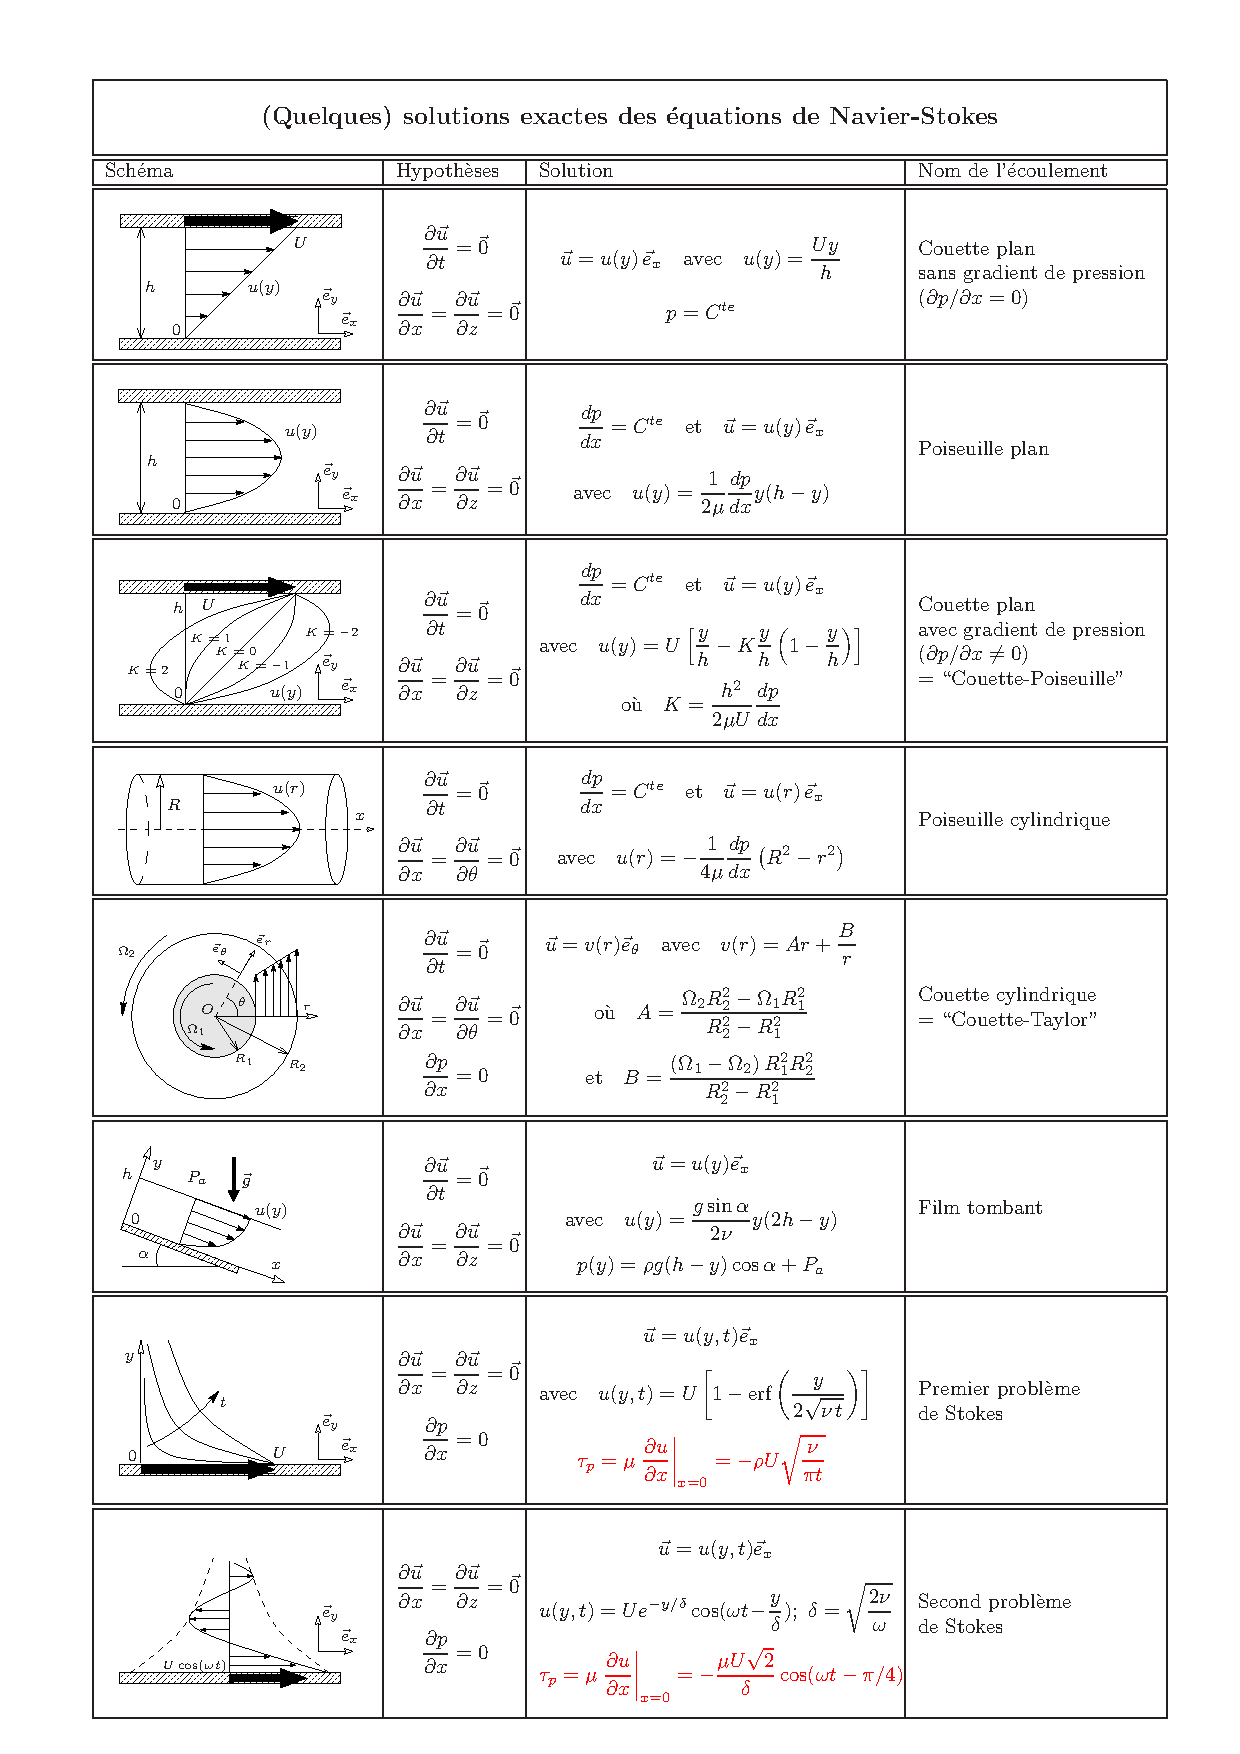
\includegraphics[height=27cm]{solutions_exactes_D}}
	\end{picture}
\end{center}


